\subsubsection{Phase 1}
In this phase we transform every $q_i \in Q$ to sequences of game blocks. These sequences will be part of the block states $P_1, \ldots P_n$ in the constructed \textit{k-cleared-cells} instance. The transformation is done by creating a sequence of 1 $\mathbf{H}_{H}$, $q_i$ $\mathbf{H}$ and 1 $\mathbf{H}_H$ blocks (in their initial state) for each give $q_i$.

\begin{figure}[H]
    \centering
    \resizebox{0.4\textwidth}{!}{
    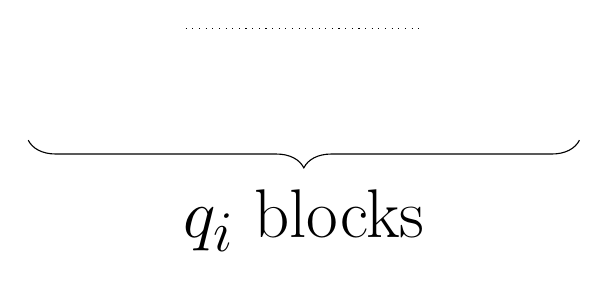
\begin{tikzpicture}
        \startb{0}{0}
        \middleb{3}{0}
        \draw[dotted] (5, 1) -- (8, 1);
        \middleb{8}{0}
        \startb{11}{0}
        \draw [decorate,decoration={brace,amplitude=10pt,mirror},xshift=0pt,yshift=-12pt]
        (3, 0) -- (10, 0) node [below,black,midway,yshift=-0.5cm]
        {\Huge $q_i$ blocks};
    \end{tikzpicture}
    }
    \caption{Transformation of \textit{Subset sum} element $q_i$}
    \label{fig:wells}
\end{figure}

When placing the first block it is evident that we have only two choices: place the $\mathbf{H}_H$ block column 2-3 of any well. This transform the chosen well from a closed to an open state. We then proceed to placing the middle $q_i$ blocks. When deciding the outcome of these placements the following lemmas are of use:\\

\begin{lem}
TODO: prove that the height doesn't change in the columns in phase 1. Important for second lemma.
\end{lem}

\bigbreak

\begin{lem}
\label{lem:permclose}
In phase 1, placing a $\mathbf{H}$ block in any other column than 4-5 in a well will make the same well permanently closed.
\end{lem}

\begin{proof}
In the first case, the well is closed. We can only place the $\mathbf{H}$ block in column 2-3. Since no cells are cleared as a result, column 1 to 4 are filled except for the top two rows. We therefore cannot place any block in these columns without a game over. Either the column right of column 5 is filled, or the gameboard has ended. Since column 4 is also filled, we cannot place any block in column 5. Thus the well is permanently closed.

In the second case, the well is open. Apart from column 4-5, the $\mathbf{H}$ block can only be placed in column 3-4. This does not clear any cells as a result. Thus with the same arguments as in the first case, the well is permanently closed.
\end{proof}

Since later in the proof it will become apparent that having a permanently closed well makes it impossible to construct a optimal trajectory sequence, lemma~\ref{lem:permclose} leaves us no choice but to place all $\mathbf{H}$ blocks in column 4-5 of the open well. Finally the last $\mathbf{H}_H$ block must be placed either in column 2-3 of a closed well, or column 3-4 of an open well, in order to not permanently close a well.

\begin{figure}[H]
    \centering
    \begin{subfigure}[b]{0.55\textwidth}
        \resizebox{\linewidth}{!}{
            \begin{tikzpicture}
                \welldefault{0}{0}
                \startb{1}{10}
                \welldefault{5}{0}
                \draw[dashed] (0, 0) -- (0, 12);
                \draw[dashed] (10, 0) -- (10, 12);
                \draw[dashed] (0, 0) -- (10, 0);
                \draw[->, line width=10pt] (11, 6) -- (14, 6);
                \wellopenwhole{15}{0}
                \welldefault{20}{0}
                \draw[dashed] (15, 0) -- (15, 12);
                \draw[dashed] (25, 0) -- (25, 12);
                \draw[dashed] (15, 0) -- (25, 0);
            \end{tikzpicture}
        }
        \caption{First block}
    \end{subfigure}

    \begin{subfigure}[b]{0.55\textwidth}
        \resizebox{\linewidth}{!}{
            \begin{tikzpicture}
                \wellopenwhole{0}{0}
                \middleb{3}{10}
                \welldefault{5}{0}
                \draw[dashed] (0, 0) -- (0, 12);
                \draw[dashed] (10, 0) -- (10, 12);
                \draw[dashed] (0, 0) -- (10, 0);
                \draw[->, line width=10pt] (11, 6) -- (14, 6);
                \wellopenwhole{15}{0}
                \cellw{18}{7}
                \cellw{18}{6}
                \welldefault{20}{0}
                \draw[dashed] (15, 0) -- (15, 12);
                \draw[dashed] (25, 0) -- (25, 12);
                \draw[dashed] (15, 0) -- (25, 0);
            \end{tikzpicture}
        }
        \caption{Middle blocks}
    \end{subfigure}

    \begin{subfigure}[b]{0.55\textwidth}
        \resizebox{\linewidth}{!}{
            \begin{tikzpicture}
                \wellopenwhole{0}{0}
                \cellw{3}{7}
                \cellw{3}{6}
                \startb{2}{10}
                \welldefault{5}{0}
                \draw[dashed] (0, 0) -- (0, 12);
                \draw[dashed] (10, 0) -- (10, 12);
                \draw[dashed] (0, 0) -- (10, 0);
                \node at (12.5, 6)
                {\Huge or};
                \wellopenwhole{15}{0}
                \cellw{18}{7}
                \cellw{18}{6}
                \welldefault{20}{0}
                \startb{21}{10}
                \draw[dashed] (15, 0) -- (15, 12);
                \draw[dashed] (25, 0) -- (25, 12);
                \draw[dashed] (15, 0) -- (25, 0);
            \end{tikzpicture}
        }
        \caption{Final block}
    \end{subfigure}

    \caption{Block placement in phase 1}
    \label{fig:placement}
\end{figure}

Assuming that no blocks has been place such that any well is permanently closed, the following invariants holds at the start of the sequence corresponding to $q_i$:

\begin{enumerate}
\item Either both of the wells are closed, or both of the wells are open.

\item Column 1, 3 and 5 in any well are unchanged from the initial gameboard. Column 2 is unchanged except from the top two rows (which may be black or empty).

\item Let $q_0 = 0$. This does not change the semantics of the givet \textit{Subset sum} instance. Then in total 
\begin{equation*}
    2 \left( i-1 \right) + \sum_{j=0}^{i-1} q_j
\end{equation*}
blocks has been placed.

\item Since each block placement clears exactly 4 cells
\begin{equation*}
    8 \left( i-1 \right) + 4 \sum_{j=0}^{i-1} q_j
\end{equation*}
cells has been cleared.

\item There exists: 
    \begin{equation*}
        M_1, M_2 \subseteq \{q_0, \ldots q_{i-1}\}, M_1 \cap M_2 = \varnothing, M_1 \cup M_2 = \{q_0, \ldots, q_{i-1}\}
    \end{equation*}
such that for any well $w \in \{1,2\}$ it holds that the rows in interval
    \begin{equation*}
        \left[ 2 \left( K-1 + \sum Q - \sum M_w \right) +1, 2 \left( K-1 + \sum Q \right) \right]
    \end{equation*}
consists of white cells in column 4, and the rows in interval
    \begin{equation*}
        \left[ 1, 2 \left( K-1 + \sum Q - \sum M_w \right) \right]
    \end{equation*}
consists of black cells in column 4.
\end{enumerate}

\begin{figure}[H]
    \centering
    \resizebox{!}{0.3\paperheight}{
    \begin{tikzpicture}
        \invariantchart{0}{0}
        \draw[dashed] (-1, 0) -- (6, 0);
        \draw[dashed] (-1, 6) -- (6, 6);
        \draw[dashed] (-1, 12) -- (6, 12);
        \draw[dashed] (-1, 20) -- (6, 20);
        \draw[dashed] (5, 0) -- (5, 22);
        \draw [decorate,decoration={brace,amplitude=10pt},xshift=-12pt,yshift=0pt]
        (0, 0) -- (0, 6) node [left,align=right,black,midway,xshift=-1cm]
        {\huge $2 \left( K-1 \right)$ rows};
        \draw [decorate,decoration={brace,amplitude=10pt},xshift=-12pt,yshift=0pt]
        (0, 6) -- (0, 12) node [left,align=right,black,midway,xshift=-1cm]
        {\huge $2 \left( \sum Q - \sum M_w \right)$ rows};
        \draw [decorate,decoration={brace,amplitude=10pt},xshift=-12pt,yshift=0pt]
        (0, 12) -- (0, 20) node [left,align=right,black,midway,xshift=-1cm]
        {\huge $2 \sum M_w $ rows};
    \end{tikzpicture}
    }
    \caption{Depiction of invariants}
    \label{fig:invariant}
\end{figure}

